%%%%%%%%%%%%%%%%%%%%%%%%%%%%%%%%%%%%%%%%%%%%%%%%%
% Chapter: Introduction
%%%%%%%%%%%%%%%%%%%%%%%%%%%%%%%%%%%%%%%%%%%%%%%%%
\chapter{Introduction}
\label{chap:intro}

\ac{PMIx} is an application programming interface standard that provides
libraries and programming models with portable and well-defined access to commonly
needed services in distributed and parallel computing systems.
A typical example of such a service is the portable and scalable exchange of network
addresses to establish communication channels between the processes of a parallel
application or service.
As such, \ac{PMIx} gives distributed system software providers a better understanding of how
programming models and libraries can interface with and use system-level services.
As a standard, \ac{PMIx} provides \acp{API} that allow for
portable access to these varied system software services and the
functionalities they offer.  Although these services can be defined and implemented directly by the
system software components providing them, the
community represented by the \ac{ASC}
feels that the development of a shared standard better serves the
community.
As a result, \ac{PMIx} enables programming languages and libraries to focus on their core
competencies without having to provide their own system-level services.

%%%%%%%%%%%%%%%%%%%%%%%%%%%%%%%%%%%%%%%%%%%%%%%%%
%%%%%%%%%%%%%%%%%%%%%%%%%%%%%%%%%%%%%%%%%%%%%%%%%
\section{Background}
\label{chap:introduction:background}

The \ac{PMI} has been used for quite some time as a means of exchanging wireup information needed for inter-process communication.
Two versions (PMI-1 and PMI-2 \cite{2010-Balaji-EuroMPI}) have been released as part of the MPICH effort, with PMI-2 demonstrating better scaling properties than its PMI-1 predecessor.

PMI-1 and PMI-2 can be implemented using \ac{PMIx} though \ac{PMIx} is not a strict superset of either.
Since its introduction, \ac{PMIx} has expanded
on earlier \ac{PMI} efforts by
providing an extended version of the \ac{PMI} \acp{API} which provide necessary functionality for launching and managing parallel applications and tools at scale.

The increase in adoption has motivated the creation of this document to formally specify the intended behavior of the \ac{PMIx} \acp{API}.

More information about the \ac{PMIx} standard and affiliated projects can be found at the \ac{PMIx} web site: \url{https://pmix.org}

%%%%%%%%%%%%%%%%%%%%%%%%%%%%%%%%%%%%%%%%%%%%%%%%%
%%%%%%%%%%%%%%%%%%%%%%%%%%%%%%%%%%%%%%%%%%%%%%%%%
\section{PMIx Architecture Overview}
\label{chap:intro:arch_overview}

The presentation of the \ac{PMIx} \acp{API} within this document makes some
basic assumptions about how these \acp{API}
are used and implemented.  These assumptions are generally made only to simplify
the presentation and explain \ac{PMIx} with the expectation that most readers
have similar concepts on how computing systems are organized today.  However, ultimately
this document should only be assumed to define a set of \acp{API}.

A concept that is fundamental to \ac{PMIx} is that a \ac{PMIx} implementation might
operate primarily as a \textit{messenger}, and not a \textit{doer} --- i.e., a \ac{PMIx}
implementation might rely heavily or fully on other software components to provide
functionality~\cite{2017-Castain-EuroMPI}.
Since a \ac{PMIx} implementation might only deliver requests and responses to other
software components, the \ac{API} calls include ways to provide arbitrary information to the
backend components that actually
implement the functionality.  Also, because \ac{PMIx} implementations generally rely heavily
on other system software, a PMIx implementation might not be able to guarantee that a feature
is available on all platforms the implementation supports.  These aspects are discussed in
detail in the remainder of this chapter.

\begingroup
\begin{figure*}[ht!]
  \begin{center}
    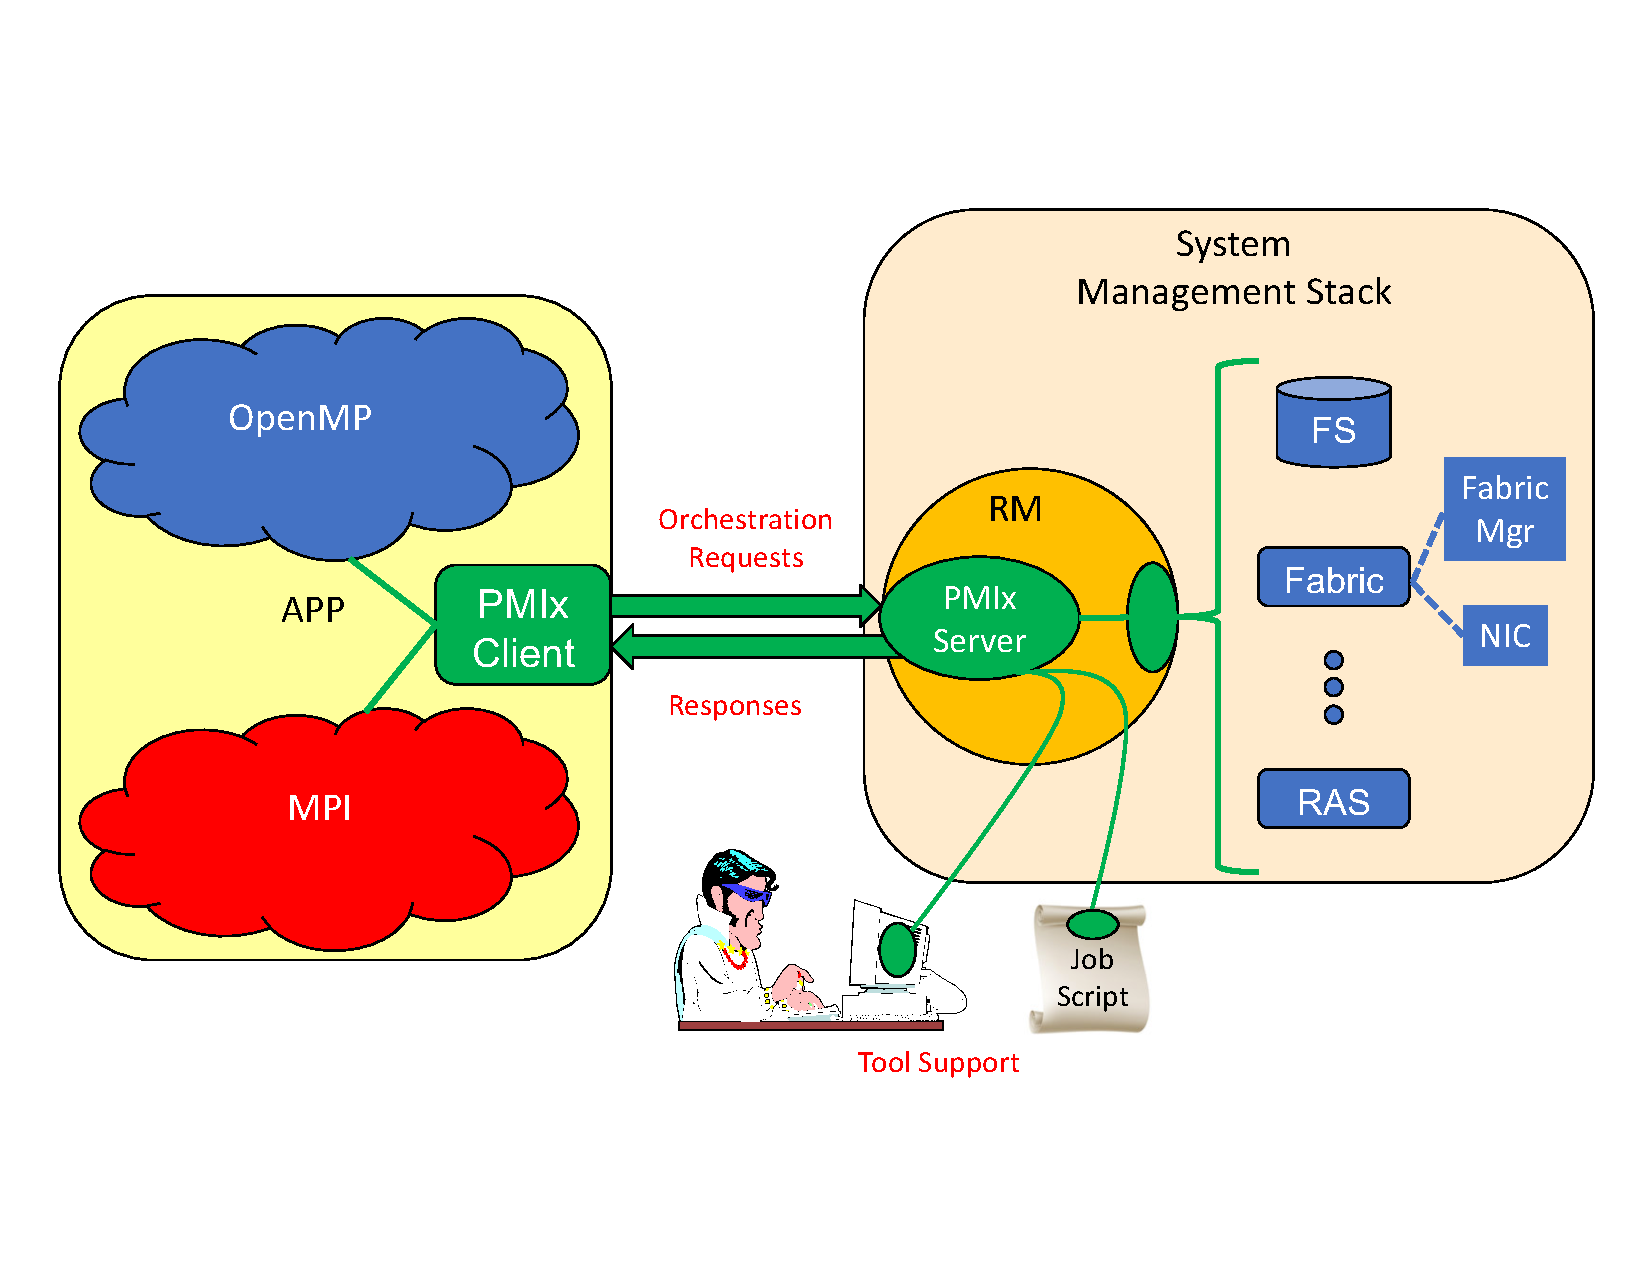
\includegraphics[clip,width=0.8\textwidth]{figs/PMIxRoles.pdf}
  \end{center}
  \caption{PMIx-SMS Interactions}
  \label{fig:roles}
\end{figure*}
\endgroup


Fig.~\ref{fig:roles} shows a typical \ac{PMIx} implementation in which the application is
built against a \ac{PMIx} client library that contains the client-side \acp{API},
attribute definitions, and communication support for interacting with the local \ac{PMIx} server.
\ac{PMIx} clients are processes which are started through the \ac{PMIx} infrastructure,
either by the PMIx implementation directly or through a \ac{SMS} component, and have registered
as clients.  A \ac{PMIx} client
is created in such a way that the \ac{PMIx} client library
will be have sufficient information available to
authenticate with the \ac{PMIx} server.
The \ac{PMIx} server will have sufficient knowledge about the
process which it created, either directly or through other \ac{SMS}, to authenticate the
process and provide information the process requests such as its identity and the
identity of its peers.

As clients invoke \ac{PMIx} \acp{API}, it is possible that some client requests can
be handled at the client level.  Other requests might require communication with the
local \ac{PMIx} server, which subsequently might request services from the host \ac{SMS}
(represented here by a \ac{RM} daemon).
The interaction between the \ac{PMIx} server and \ac{SMS} are
achieved using callback functions registered during server initialization.
The host \ac{SMS} can indicate its lack of support for any operation by simply providing a \textit{NULL} for the associated callback function, or can create a function entry that returns \textit{not supported} when called.

Recognizing the burden this places on SMS vendors, the PMIx community has included interfaces by
which the host \ac{SMS} (containing the local PMIx service instance) can request support from local \ac{SMS} elements via the PMIx API.  Once the \ac{SMS} has transferred the request to
an appropriate location, a \ac{PMIx} server interface can be used to pass the request
between \ac{SMS} subsystems.
For example, a request for network traffic statistics can utilize the
PMIx networking abstractions to retrieve the information from the Fabric Manager.
This reduces the portability and
interoperability issues between the individual subsystems by transferring the burden of defining the
interoperable interfaces from the \ac{SMS} subsystems to the \ac{PMIx} community, which continues
to work with those providers to develop the necessary support.

Fig.~\ref{fig:roles} shows how tools can interact with the \ac{PMIx} architecture.
Tools, whether standalone or embedded in job scripts, are an exception to
the normal client registration process.   A process can register as a tool, provided
the \ac{PMIx} client library has adequate rendezvous information to connect to the appropriate
\ac{PMIx} server (either hosted on the local machine or on a remote machine).  This allows processes
which were not created by the PMIx infrastructure to request access to PMIx functionality.

%%%%%%%%%%%%%%%%%%%%%%%%%%%%%%%%%%%%%%%%%%%%%%%%%
%%%%%%%%%%%%%%%%%%%%%%%%%%%%%%%%%%%%%%%%%%%%%%%%%
\section{Portability of Functionality}
\label{chap:intro:not_supported}

It is difficult to define a portable \ac{API} that will provide access to the many
and varied features underlying the operations for which \ac{PMIx} provides access.
For example, the options and features provided to request the creation
of new processes varied dramatically between different systems existing
at the time \ac{PMIx} was introduced.  Many \acp{RM} provide rich interfaces
to specify the resources assigned to processes.
As a result, \ac{PMIx} is faced with the challenge
of attempting to meet the seamingly conflicting goals of creating an \ac{API} which allows
access to these diverse features while being portable across a wide range of
existing software environments. In addition, the functionalities required by different
clients vary greatly.  Producing a \ac{PMIx} implementation
which can provide the needs of all possible clients on all of its target systems
could be so burdensome as to discourage \ac{PMIx} implementations.

To help address this issue, the \ac{PMIx} \acp{API} are designed to allow resource managers
and other system management stack components to decide on support of a
particular function and allow client applications to query and adjust to the level of support available.  \ac{PMIx} clients should be written to account for the possibility that a \ac{PMIx} \ac{API} might return an error code indicating that the call is not supported.
The \ac{PMIx} community continues to look at ways to assist \ac{SMS} implementers in their decisions
on what functionality to support by highlighting functions and attributes that are
critical to basic application execution (e.g., \refapi{PMIx_Get}) for certain classes of applications.

Attributes in this document are organized according to their primary usage, either grouped with a specific \ac{API} or included in an appropriate functional chapter. \ac{PMIx} Standard attributes all start with \code{"PMIX"} in their name, and many include a functional description as part of their name (e.g., the use of \code{"PMIX_FABRIC_"} at the beginning of fabric-specific attributes). The \ac{PMIx} Standard also defines one generalized attribute for a special purpose:

\declareAttribute{PMIX_ATTR_UNDEF}{"pmix.undef"}{NULL}{
A default attribute name signifying that the attribute field of a \ac{PMIx} structure (e.g., a \refstruct{pmix_info_t}) has not yet been defined.
}

%%%%%%%%%%%%%%%%%%%%%%%%%%%%%%%%%%%%%%%%%%%%%%%%%
\subsection{Optional Nature of Attributes}

An area where differences between support on different systems can be challenging is regarding the attributes that provide information to the client process and/or control the behavior of a \ac{PMIx} \ac{API}.  Most
\ac{PMIx} \ac{API} calls can accept additional information or attributes specified in the form of
key/value pairs. These attributes provide information to the \ac{PMIx} implementation that influence the
behavior of the \ac{API} call.  In addition to \ac{API} calls being optional, support for the
individual attributes of an \ac{API} call can vary between systems or implementations.

An application can adapt to the attribute support on a particular system in one of two ways.
\ac{PMIx} provides an \ac{API} to enable an application to query the attributes
supported by a particular \ac{API} (See \ref{chap:api_job_mgmt:queryattrs}).
Through this \ac{API}, the \ac{PMIx} implementation can provide detailed information
about the attributes supported on a system for each \ac{API} call queried.
Alternatively, the application can mark attributes as
required using a flag within the \refstruct{pmix_info_t} (See \ref{chap:struct:info}).
If the required attribute is
not available on the system or the desired value for the attribute is not available, the call will
return the error code for \textit{not supported}.

For example, the \refattr{PMIX_TIMEOUT} attribute can be used to specify the time (in seconds) before the requested operation should time out. The intent of this attribute is to allow the client to avoid ``hanging'' in a request that takes longer than the client wishes to wait, or may never return (e.g., a \refapi{PMIx_Fence} that a blocked participant never enters).

The application can query the attribute support for \refapi{PMIx_Fence}
and search whether \refattr{PMIX_TIMEOUT} is listed as a supported attribute.  The application can also
set the required flag in the \refstruct{pmix_info_t} for that attribute when making the \refapi{PMIx_Fence}
call. This will return an error if this attribute is not supported. If the required flag is not set,
the library and \ac{SMS} host are allowed to treat the attribute as optional, ignoring it if support
is not available.

It is therefore critical that users and application implementers:

\begin{compactalphaenum}
\item consider whether or not a given attribute is required, marking it accordingly; and

\item check the return status on all \ac{PMIx} function calls to ensure support was present and that the request was accepted. Note that for non-blocking \acp{API}, a return of \refconst{PMIX_SUCCESS} only indicates that the request had no obvious errors and is being processed – the eventual callback will return the status of the requested operation itself.
\end{compactalphaenum}

\ac{PMIx} clients (e.g., tools, parallel programming libraries) may find that they depend only on a small subset of interfaces and attributes to work correctly.
\ac{PMIx} clients are strongly advised to define a document itemizing the \ac{PMIx} interfaces and associated attributes that are required for correct operation, and are optional but recommended for full functionality.
The \ac{PMIx} standard cannot define this list for all given \ac{PMIx} clients, but such a list is valuable to \acp{RM} desiring to support these clients.

A \ac{PMIx} implementation may be able to support only a subset of the \ac{PMIx} \acs{API} and attributes on
a particular system due to either its own limitations or limitations of the \ac{SMS} with which it interfaces.
A \ac{PMIx} implemenation may also provide additional attributes beyond those defined herein in order to allow
applications to access the full features of the underlying \ac{SMS}.
\ac{PMIx} implementations are strongly advised to document the \ac{PMIx} interfaces and associated attributes they support, with any annotations about behavior limitations.
The \ac{PMIx} standard cannot define this support for implementations, but such documentation is valuable to \ac{PMIx} clients desiring to support a broad range of systems.

While a \ac{PMIx} library implementer, or an \ac{SMS} component server, may choose to support a particular \ac{PMIx} \ac{API}, they are not required to support every attribute that might apply to it. This would pose a significant barrier to entry for an implementer as there can be a broad range of applicable attributes to a given \ac{API}, at least some of which may rarely be used.

Note that an environment that does not include support for a particular attribute/\ac{API} pair is not ``incomplete'' or of lower quality than one that does include that support. Vendors must decide where to invest their time based on the needs of their target markets, and it is perfectly reasonable for them to perform cost/benefit decisions when considering what functions and attributes to support.


%%%%%%%%%%%%%%%%%%%%%%%%%%%%%%%%%%%%%%%%%%%%%%%%%
